\documentclass[11pt]{beamer}
\usetheme{Singapore}

\usepackage[utf8]{inputenc}
\usepackage[T1]{fontenc}
\usepackage{soul}
\usepackage{graphicx}
\usepackage[normalem]{ulem}
\useunder{\uline}{\ul}{}


\graphicspath{{../../Figures/}}

\def\et{{\it et al.}}


\author{Cody Glickman \\ CPBS Update Talk}

\title{Metagenomic Exploration the Sequel: \\ Development of novel tools for viral and bacterial sequence analysis}

%\subtitle{}
%\logo{}

\date{ 
\includegraphics[height=2cm, width=2cm]{lablogo.png} \\ Nov 12th, 2018}
%\subject{}
\setbeamercovered{transparent}
\setbeamertemplate{navigation symbols}{}
\setbeamertemplate{theorems}[numbered]

\begin{document}
	\maketitle
	\begin{frame}{Research Update}
	\begin{block}{\alert{Clinical NTM Gene Databases}}
	Submitted ...
	https://mra.asm.org/latest 
	\end{block}
	
	\begin{block}{\alert{Duobiome: 18S/16S Parallel Analysis}}
	In progress
	\end{block}
	
	\begin{block}{\alert{Hybrid Viral Contig Prediction}}
	In progress
	\end{block}
	
	\begin{block}{\alert{Virulence Factors in Bacteriophages}}
	Submitted ...
	\end{block}
	\end{frame}
	
	\begin{frame}{Progress of Other Projects}
	\begin{block}{Asthma Environmental Microbiome}
	Submitted abstract to ATS
	\end{block}
	
	\begin{block}{Building Up Domains: Lysogenic Host Discovery}
	Incorporated into large collaborative NCBI initative
	\end{block}
	
	\begin{block}{Genomic Retrieval and Blast Database Creation}
	Accepted Poster ISME 2017
	\end{block}
	
	\begin{block}{Hawaiian Soil Chemistry and Culture}
	Submitted ...
	\end{block}
	

	\end{frame}
	%-----------------------------------------------------------
\section{}

	\begin{frame}{Nontuberculous Mycobacterial (NTM) Infections}
		\begin{block}{Number of Cases}
		The number of NTM cases is estimated over 100K
		\end{block}
		
		\begin{block}{Increasing Case}
		The rate of cases is estimated to grow at 8\% every year
		\end{block}
		
		
		\begin{block}{Populations at risk of developing NTM}
		\begin{itemize}
		\item Immunocompromised individuals 
		\item Patients with lung damage or malfunction 
		\item Residents of warm costal areas especially Hawaii
		%\item The Elderly 
		\end{itemize}
		\end{block} 
		
		\begin{block}
		
		\end{block}
	\vspace{-1cm}
	\tiny{Strollo SE, et al. Ann Am Thorac Soc. 2015 \\
	Adjemian J, et al. Am J Respir Crit Care Med. 2012}
	
	\end{frame}
	%----------------------------------------------------------
	\begin{frame}{Laboratory Research Methods}
	\begin{block}{Conditions for NTM Environmental Growth}
	Identifying important characteristics for NTM growth 
	\end{block}
	
	\begin{block}{Environmental Microbiome}
	Developing methods to characterize home environments
	\end{block}
	
	\begin{block}{Clinical NTM}
	\begin{itemize}
	\item Developing resources to study clinical NTM
	\item Identifying potential mechanisms of NTM transmission
	\end{itemize}
	\end{block}

	
	\end{frame}
	
	%-----------------------------------------------------------
	\begin{frame}{Viral Focus}
	
	\begin{block}{Bacteriophages (Phages)}
	Phages are DNA viruses that infect prokaryotes
	\end{block}
	
	\begin{block}{Phage Diversity}
	Investigating how phage abundance and diversity affect susceptibility to NTM lung infection
	\end{block}
	
	\begin{block}{Phage Vectors}
	Researching how phages act as carriers of bacterial genes within clinical NTM infections
	\end{block}
	
	\end{frame}
	%-----------------------------------------------------------
	\begin{frame}{Molecular Methods to Study Phages}
	\begin{columns}
	\column{0.5\textwidth}
	\begin{block}{Difficulties of phage study}
	\begin{itemize}
		\item Lack of universal marker gene
		\item Sequence heterogeneity 
		\item Misclassification in databases
	\end{itemize}
	\end{block}
		
		
	\begin{block}{Phage Isolation Methods}
	\begin{itemize}
		\item Biological filtration
		\item In silico methods
	\end{itemize}
	\end{block}
	
	\column{0.5\textwidth}
	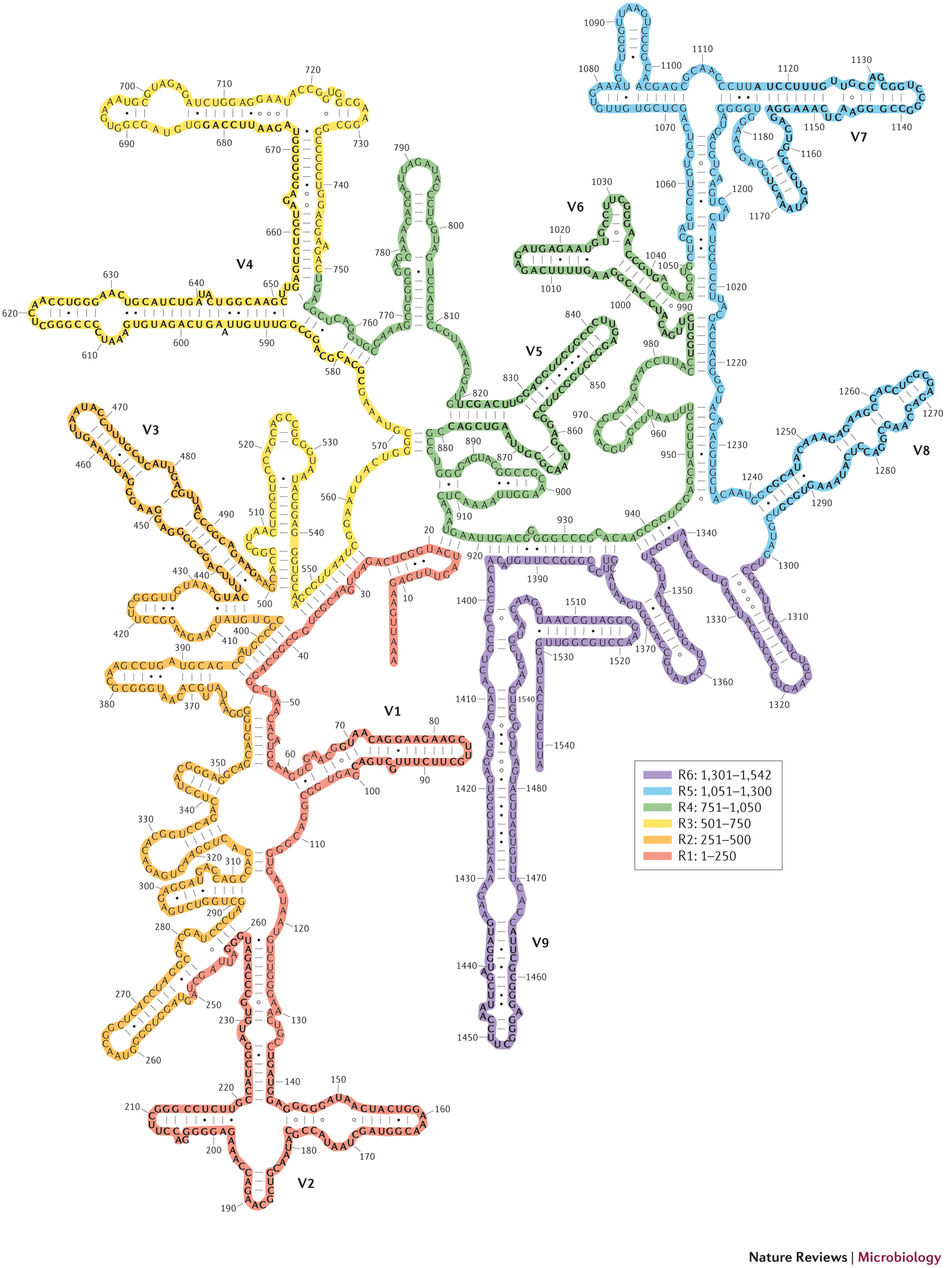
\includegraphics[height=5.5cm, width=5cm]{ribosome.jpg} \\
	\tiny{Yarza, P., et al. Nature Reviews Microbiology 2014}
	\end{columns}
		
	
	\end{frame}

	%-----------------------------------------------------------
	\begin{frame}{Objective (EDIT)}
	\center
	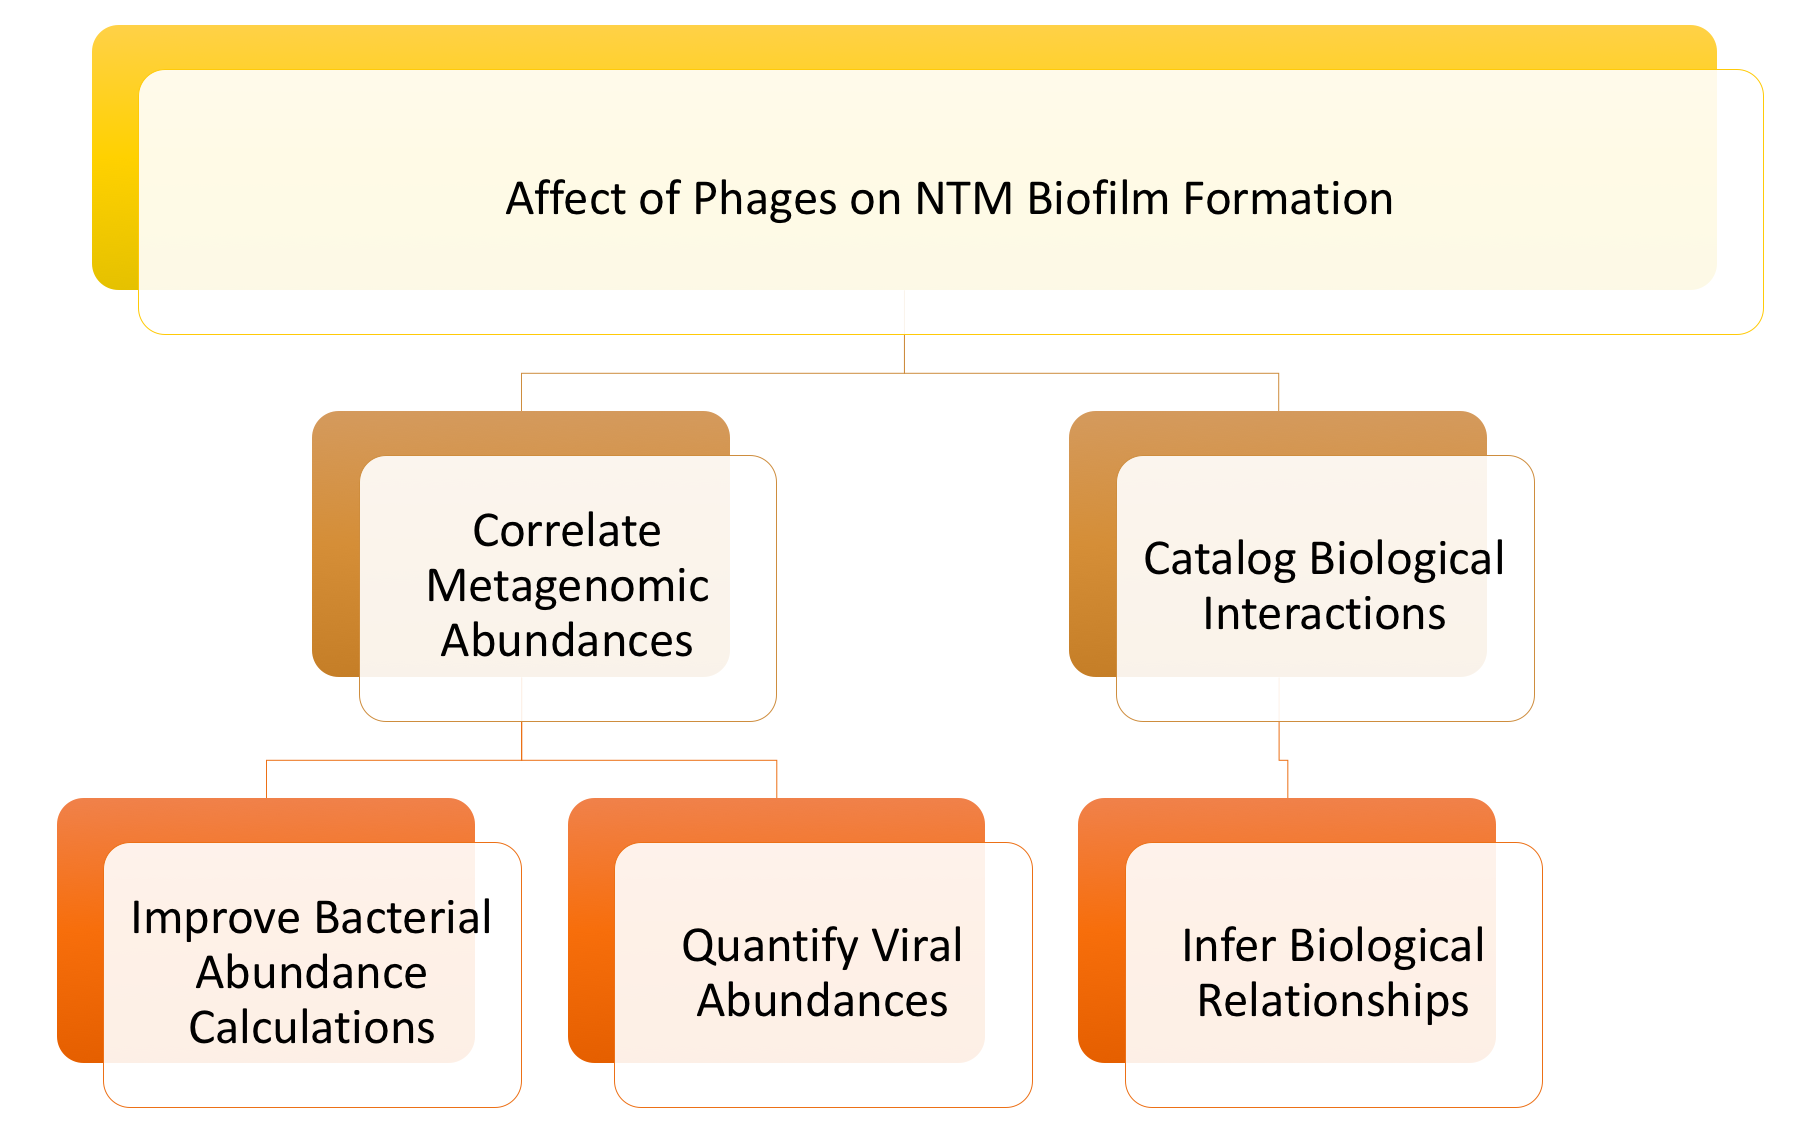
\includegraphics[height=6cm, width=9cm]{objective.png}
	
	\end{frame}

%-----------------------------------------------------------
	
\section{Clinical NTM Gene Databases}
\subsection{}
	\begin{frame}{Species Identification of NTM at NJH}
  \begin{block}{Clinical NTM Gene Database}
  Developed updated database to characterize clinical NTM
  \end{block}
	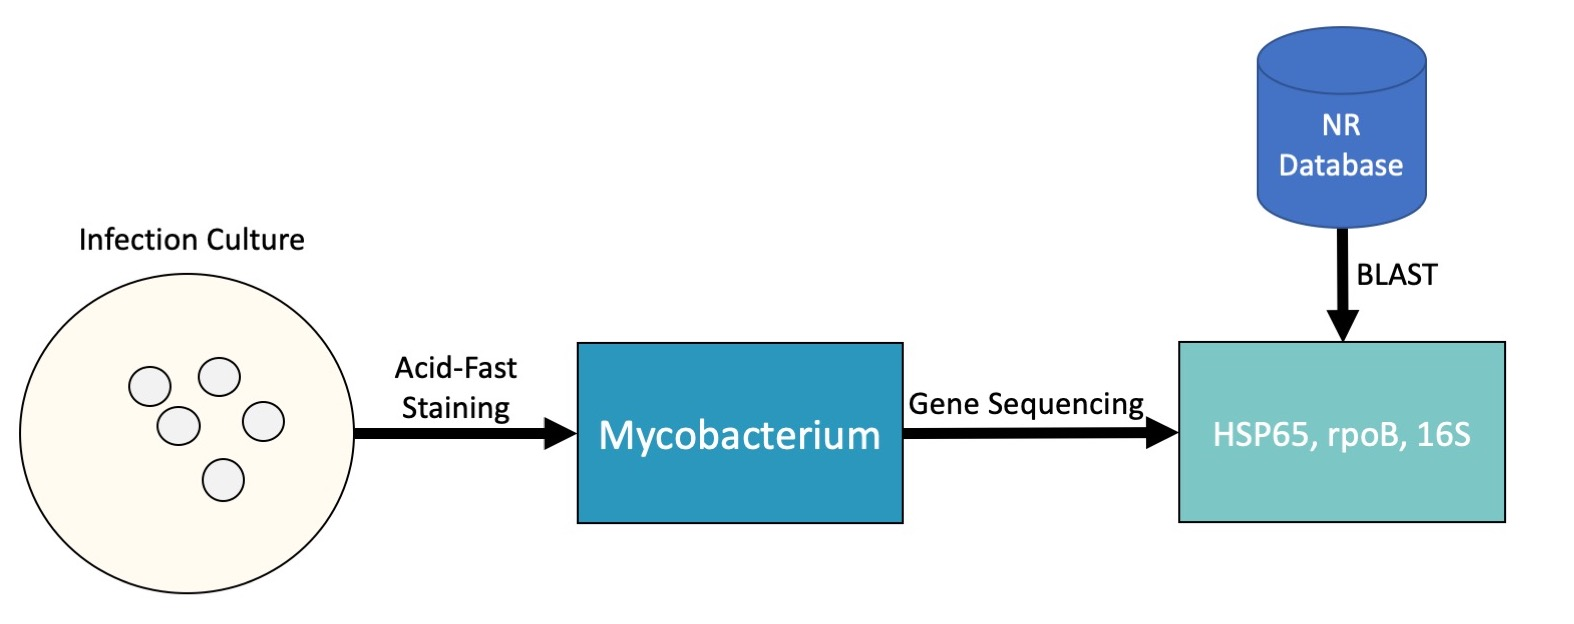
\includegraphics[height=5cm, width=11cm]{CPBS_11_18/NJH_Protocol.jpg}
	
	\end{frame}
	%-----------------------------------------------------------
	\begin{frame}{Limitations of Current Methods}
	
	\begin{columns}
	\column{0.5\textwidth}
	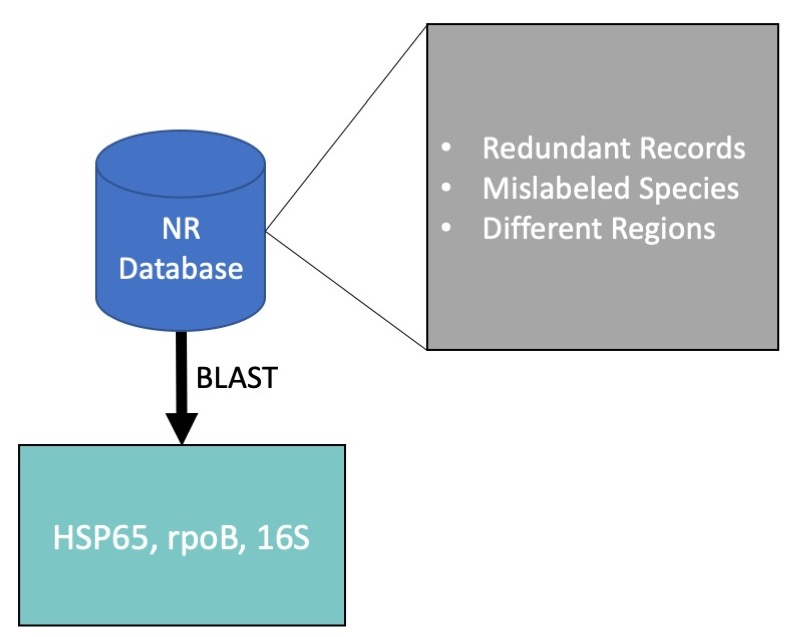
\includegraphics[height=5cm, width=5.5cm]{CPBS_11_18/Issues.jpg}
	\column{0.5\textwidth}
	\begin{block}{Redundant Records}
	Sequences between species are indistinguishable at gene
	\end{block}
	\begin{block}{Mislabeled Species}
	Naming conventions are constantly updated
	\end{block}
	\begin{block}{Different Regions}
	Current protocols amplify specific region of gene
	\end{block}
	\end{columns}
	
	%\tiny{Sczyrba, A., et al. Nature Methods 2017}
	\end{frame}
	%-----------------------------------------------------------
  \begin{frame}{Curated Gene Databases}
  \begin{block}{Number of Sequences per Species}
  The maximum number of sequences per species in the database is two
  \end{block}
  \center
  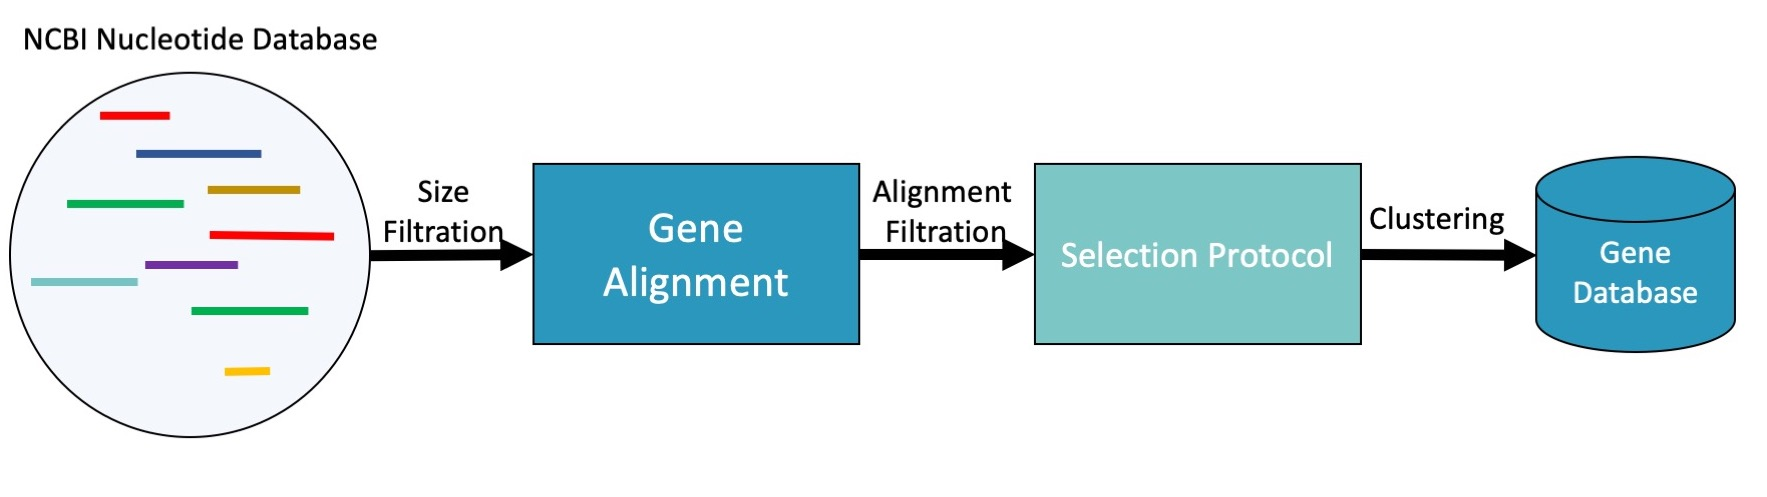
\includegraphics[height=4cm, width=11cm]{CPBS_11_18/Gene_Database_Workflow.jpg}
  \end{frame}


%-----------------------------------------------------------
  \begin{frame}{Selection Protocol}
  \center
  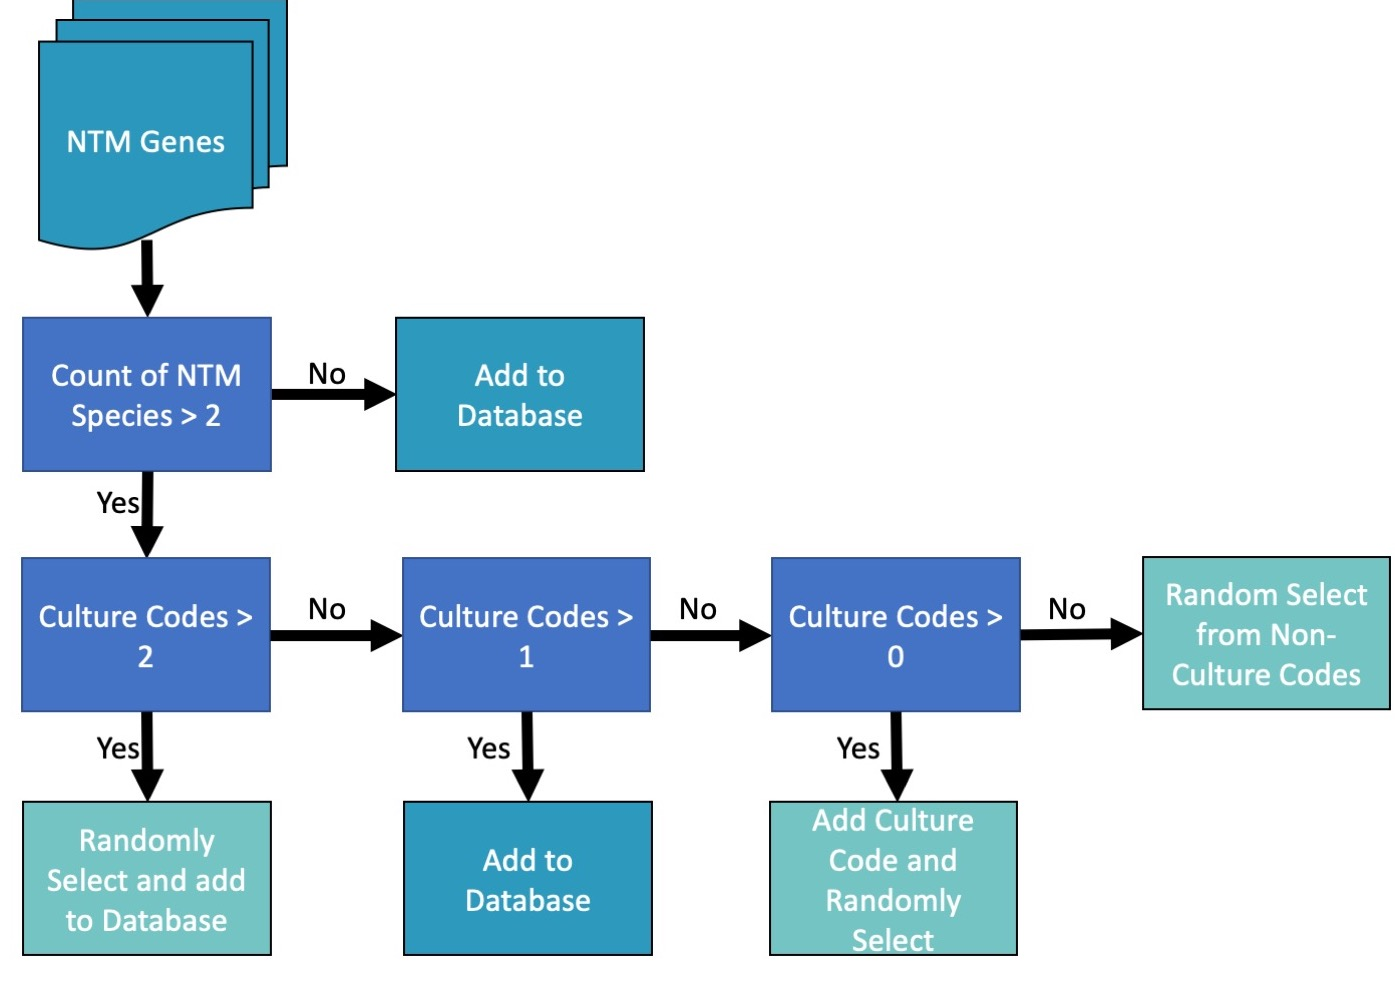
\includegraphics[height=7cm, width=11cm]{CPBS_11_18/Selection_Protocol.jpg}
  \end{frame}
%-----------------------------------------------------------
  \begin{frame}{Clinical Gene Databases}
  \begin{table}[]
  \begin{tabular}{|l|l|l|}
  \hline
  {\ul \textbf{Gene}} & {\ul \textbf{Region Size}} & {\ul \textbf{Unique Species}} \\     \hline
  hsp65 & 382 bases & 185 \\ \hline
  rpoB & 657 bases & 134 \\ \hline
  16s rRNA & 1470 bases & 184 \\ \hline
  \end{tabular}
  \caption{Table 1 highlights the regions lengths and size of the respective databases}
  \label{Test_Table}
  \end{table}
  \end{frame}
%-----------------------------------------------------------
	\begin{frame}{Database Validation}
	\begin{block}{hsp65}
	154 Species of HSP65 Validation against Subsetted Database
	96.73\% identical match 
	5 non matches - two hits in top 5
	- two hits not in database (outdated names?)
	
	\end{block}
	
	
	\tiny{Dai, J, et al. J Clin Microbiol. 2011}
	\end{frame}
	

	%-----------------------------------------------------------
	\begin{frame}{rpoB-hsp65 Tree}
	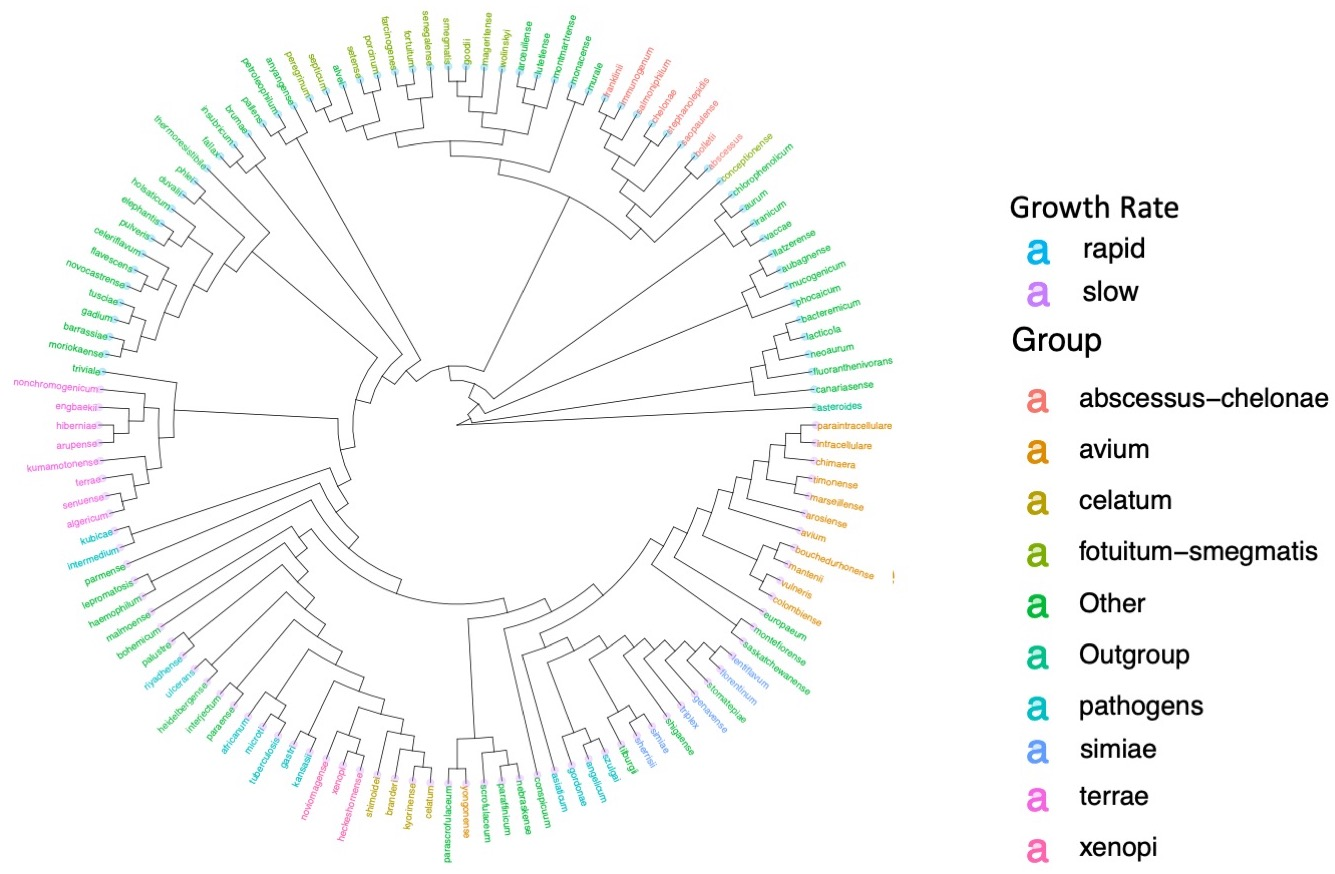
\includegraphics[height=8cm, width=11cm]{CPBS_11_18/Tree2.jpg}
	\end{frame}

%-----------------------------------------------------------
	\begin{frame}{Conclusions and Future Directions}
	
	\begin{block}{Representation}
	The subsetted database is highly representative of prior published works
	\end{block}
	
	\begin{block}{Benefits of Curated Database}
	\begin{itemize}
	\item Aligned sequences to shared region
	\item Preferentially selected established culture codes
	\item Condensed and explicitly labeled ambiguous sequences 
  \end{itemize}
	\end{block}
	
	\begin{block}{Limitations}
	Size of the gene sequence databases may not differentiate between species
	\end{block}
	
	\tiny{Dai, J, et al. J Clin Microbiol. 2011 \\ Tortoli}
  \end{frame}
	
%-----------------------------------------------------------

\section{Duobiome}
\subsection{}

	
	\begin{frame}{Microbiome}
	\begin{columns}
	\column{0.5\textwidth}
	\begin{block}{16S Ribosomal RNA Sequencing}
	\begin{itemize}
		\item Amplifies a region of gene
		\item Community level analysis 
	\end{itemize}
	\end{block}
		
		
	\begin{block}{Traditional Limitations}
	\begin{itemize}
		\item Biological filtration
		\item In silico methods
	\end{itemize}
	\end{block}
	
	\column{0.5\textwidth}
	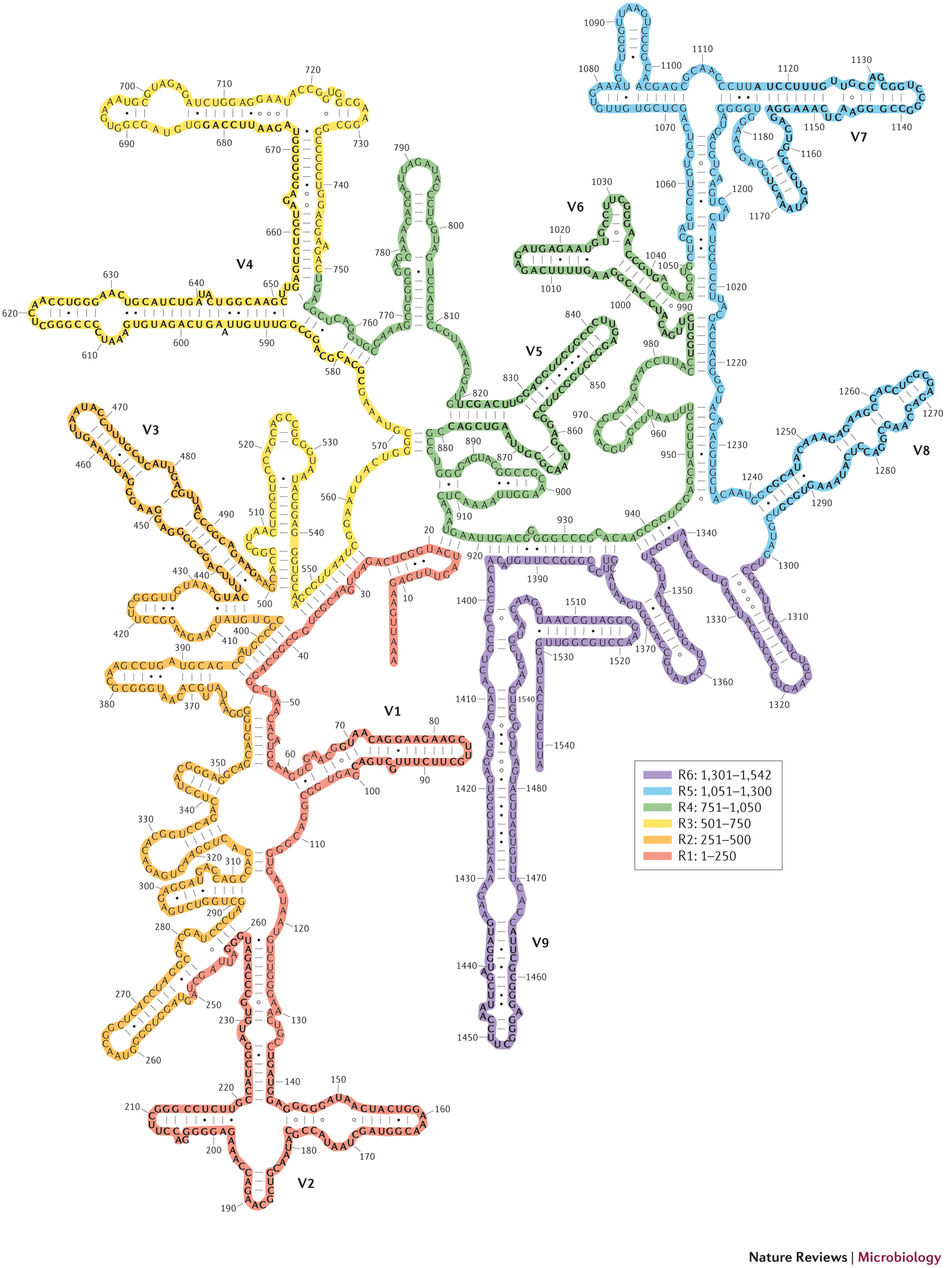
\includegraphics[height=5.5cm, width=5cm]{ribosome.jpg} \\
	\tiny{Yarza, P., et al. Nature Reviews Microbiology 2014}
	\end{columns}
		
	
	\end{frame}
	%-----------------------------------------------------------
	\begin{frame}{Degenerate Primers}
	\begin{columns}
	
	
	\column{0.5\textwidth}
	\begin{block}{Degenerate Primer Example}
	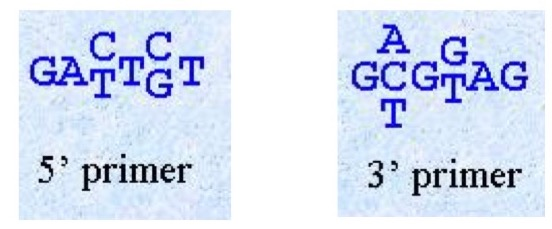
\includegraphics[height=3cm, width=5cm]{CPBS_11_18/primers.jpg}
	\end{block}
	\column{0.5\textwidth}
	\begin{block}{Feature of Degenerate Primers}
	Dual amplification of eukaryotic (18S) and prokaryote (16S)
	\end{block}
	\begin{block}{Universal 16S/18S Primer}
	515F - 806R primer
	\end{block}
	\end{columns}
	\tiny{Caporaso, J.G., et al. PNAS 2011 \\ Wang, Y., et al. PLOS One 2014}

	\end{frame}
	%-----------------------------------------------------------
	
	\begin{frame}{Analyze both}
	
	\end{frame}
	%-----------------------------------------------------------
	
	
	\begin{frame}{Testing against BLAST based and traditional pipeline}
	
	\end{frame}
	%-----------------------------------------------------------
	
	%-----------------------------------------------------------
	\begin{frame}{Future Directions}
	\begin{block}{Webserver}
	Shiny web application in development
	\end{block}
	
	\begin{block}{Viral GRAB}
	\begin{itemize}
	\item Expansion of GRAB to viral elements
	\item Features include ability to filter viruses by genetic material type
	\end{itemize}
	\end{block}
	\end{frame}
	
	

\section{Virulence Factors in Bacteriophages}
\subsection{}
	
	\begin{frame}{Virulence}
		\begin{block}{Virulence Defined}
		The capacity of a microorganism to proliferate despite host defenses
		\end{block}
		
		\begin{block}{Influences on Virulence}
		\begin{itemize}
		\item Number of microorganisms
		\item \alert{Composition of the mobile genetic reservoir}
		\item Location of niche
		\item Host immune capabilities
		\end{itemize}
		\end{block}
	
	\end{frame}
	%--------------------------------------------------------------------------------------

	\begin{frame}{Bacterial Virulence Factors Increase Pathogenesis}
	\begin{columns}
	\column{0.65\textwidth}
	\begin{block}{Examples of Virulence Factors}
		\begin{itemize}
		\item Increased fitness for nutrients
		\item Host immunity resistance
		\item Toxin secretion
		\end{itemize}
	\end{block} 
	
	\begin{block}{Diseases from Virulence Factors}
	Cholera, dysentery, botulism, and food poisoning
	\end{block}
	

	\column{0.4\textwidth}
	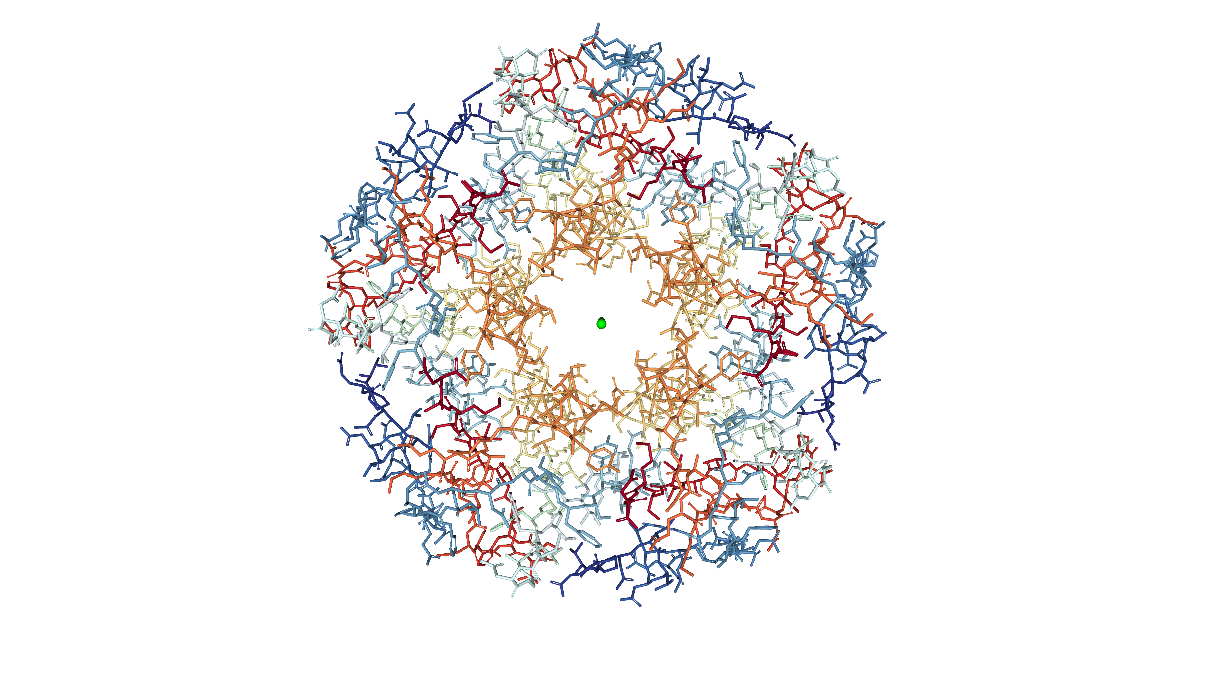
\includegraphics[height=3cm, width=5cm]{cholera.png}

	\vspace{-0.3cm}
	\hspace{0.5cm}	
	\tiny{PDB Structure of Cholera Toxin}
	\end{columns}
	
	\end{frame}
	
	%--------------------------------------------------------------------------------------
	
	\begin{frame}{Bacteriophages as a Genetic Reservoir \\ of Virulence Factors Genes}
	\begin{columns}
	\column{0.5\textwidth}
	\begin{block}{Bacteriophages (Phages)}
	DNA viruses that infect bacteria
	\end{block}
	
	
	\begin{block}{Phages and Pathology}
	Virulence Factors that cause cholera, dysentery, botulism, and food poisoning are carried on phage elements.
	\end{block}
	
	\column{0.5\textwidth}
	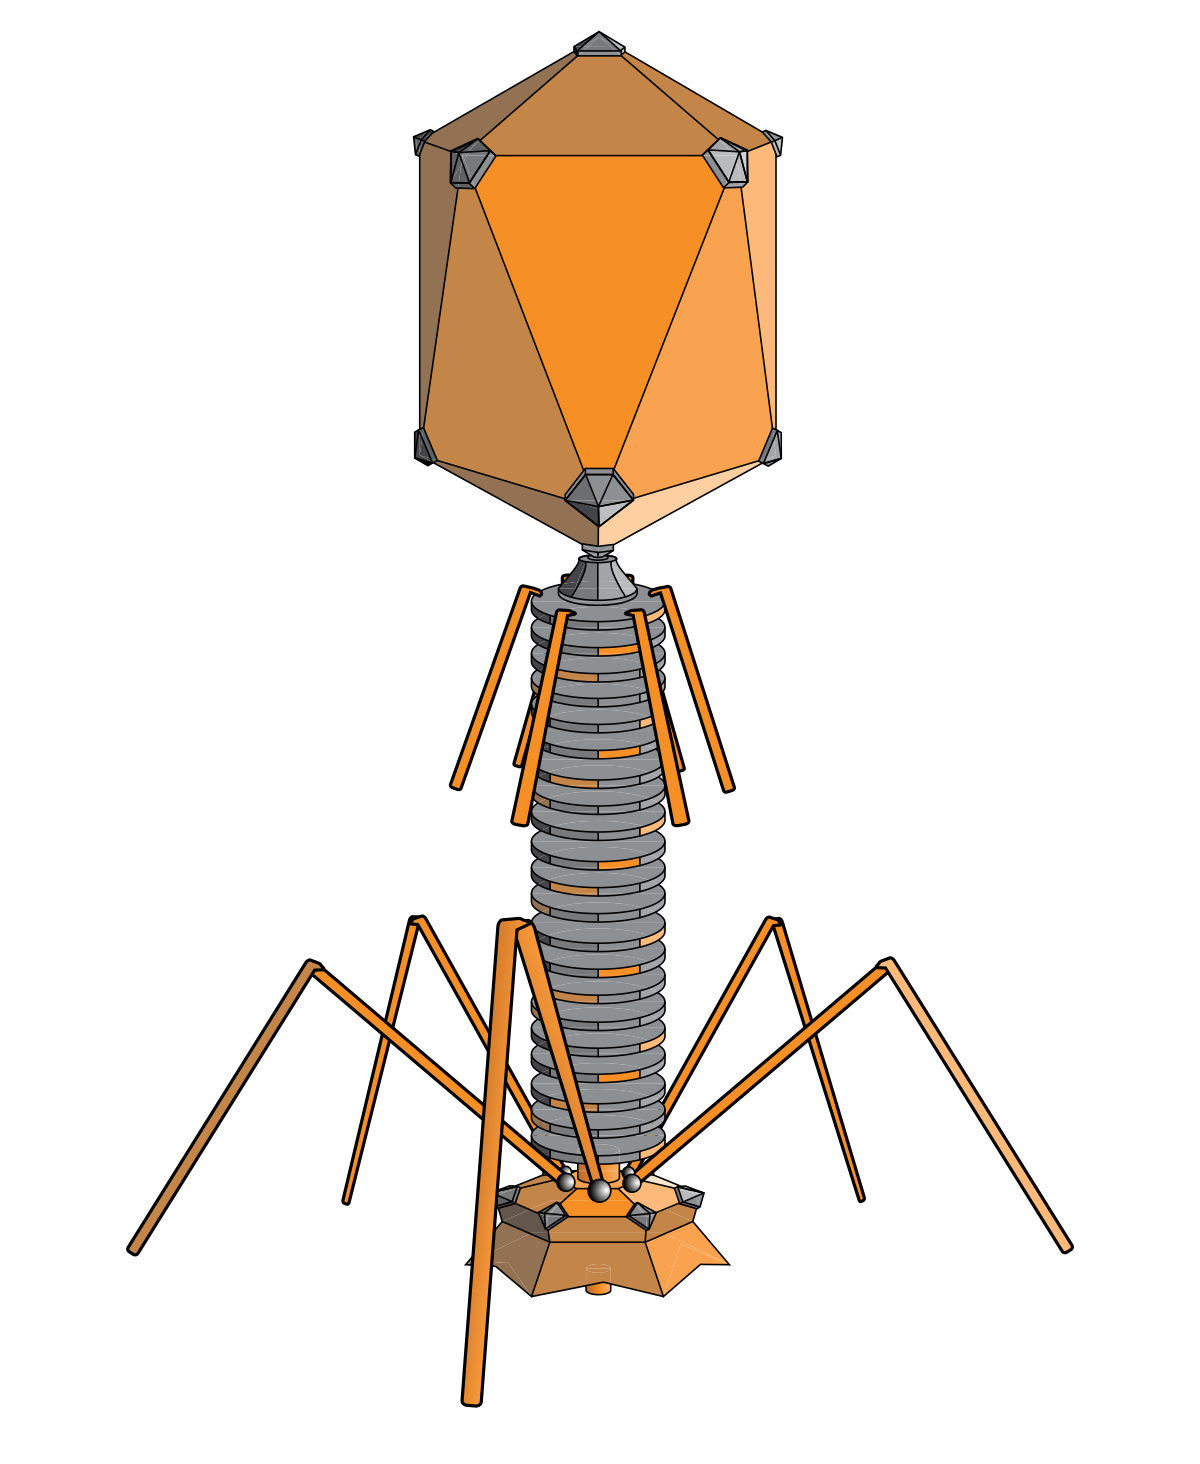
\includegraphics[height=5.5cm, width=5cm]{phage.png} \\
	\hspace{0.5cm}	
	\tiny{Novick, Richard, Plasmid (2003)}
	\end{columns}
	
	\begin{block}{Objective}
	Characterize the abundance of bacterial virulence factors in phages
	\end{block}
	
	\end{frame}

	
\section{Establishing Baseline Virulence Factor Abundance}
\subsection{}


	%-----------------------------------------	
	\begin{frame}{Data}
	\begin{columns}
	\column{0.5\textwidth}
	\begin{block}{Virulence Protein Databases}
		\begin{itemize}
			\item VFDB \\ \tiny{Chen, Lihong, et al. Nucleic Acids Research (2005)}
			\item \large{PatricVF} \\ \tiny{Wattam, AR, et al. Nucleic Acids Research (2017)}
		\end{itemize}
	\end{block}
	\begin{block}{Virulence HMMs}
	\begin{itemize}
		\item pFam \\ \tiny{Bateman, Alex, et al. Nucleic Acids Research (2004)}
		\item \large{pVOG} \\ \tiny{Grazziotin, AL, et al. Nucleic Acids Research (2016)}
	\end{itemize}
	\end{block}
	
	
	\column{0.5\textwidth}
	\begin{block}{Phage Protein Database}
	
\includegraphics[height=3cm, width=3cm]{uniprot.png}
	\end{block}
	\end{columns}
	\end{frame}

	%-----------------------------------------	
	\begin{frame}{Methods}
	\begin{columns}
	\column{0.7\textwidth}
	\begin{block}{Sequence Annotation Methods}
	BLAST vs \alert{HMM}
	\end{block}
	
	\begin{block}{Normalizing By Gene Count}
	Hit Percentage = $P$ \\
	Hit Count = $HC$ \\
	Gene Count = $GC$ \\
	\vspace{0.3cm}
	\hspace{1.5cm}	
	$P = {HC}/{GC}$
	\end{block}
	
	\begin{block}{Filtering By Phage Abundance}
	\alert{Streptococcus} phage: \\
	Genera abundance greater than 30
	\end{block}
	
	
	
	\column{0.2\textwidth}
	\hspace{-2cm}
	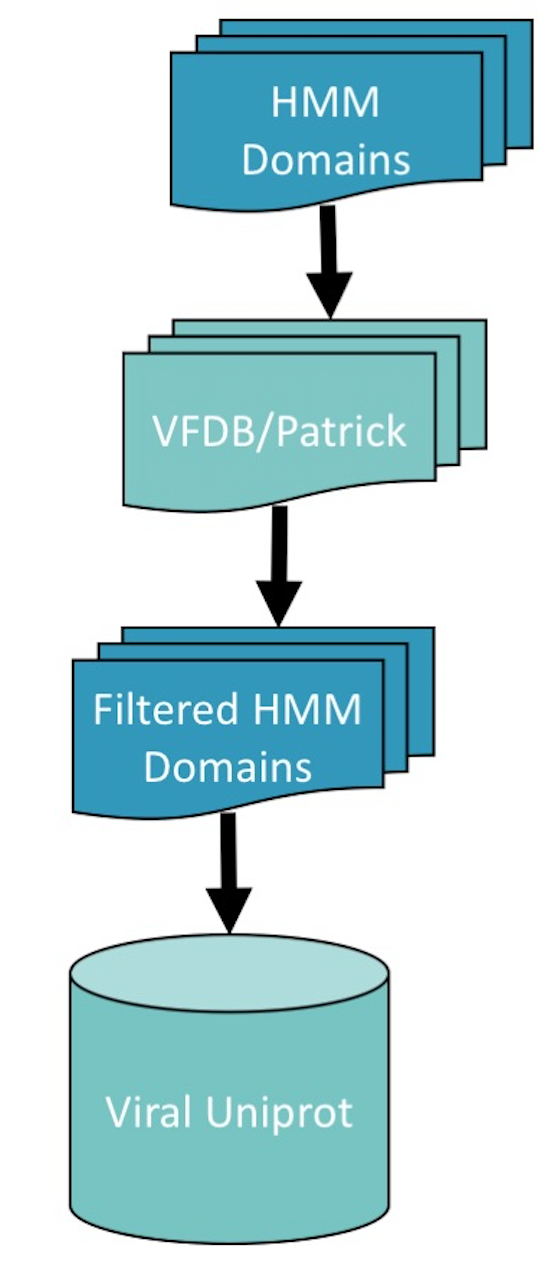
\includegraphics[height=6cm, width=3cm]{Pipeline.png}

	\end{columns}
	\end{frame}
	
	
	%-----------------------------------------	
	\begin{frame}{HMM Hit Distribution}
	\begin{columns}
	\column{0.6\textwidth}
	% Need to place figure
	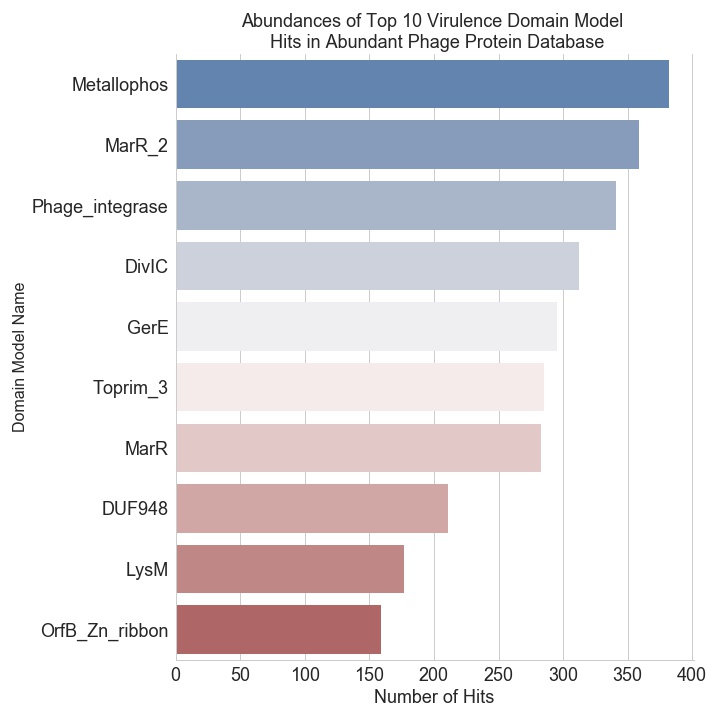
\includegraphics[height=6cm, width=6cm]{Abundant_Phages_HMM_ID.jpg}
	\column{0.5\textwidth}
	\begin{block}{MarR}
	Domain involved in antibiotic resistance
	\end{block}
	\begin{block}{DivIC}
	Part of sporulation process
	\end{block}
	\begin{block}{LysM}
	General peptidoglycan function
	\end{block}
	\end{columns}
	\end{frame}
	
	%-----------------------------------------	
	\begin{frame}{Distribution of Hit Percentage in All Phages}
	\centering
	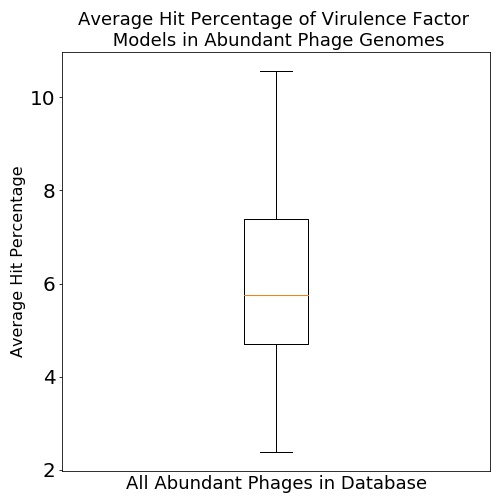
\includegraphics[height=7cm, width=7cm]{Abundant_Phages_Percentage.jpg}
	
	\end{frame}
	
	%-----------------------------------------	
	\begin{frame}{Abundant Phage Distributions by Genera Name}
	\centering
	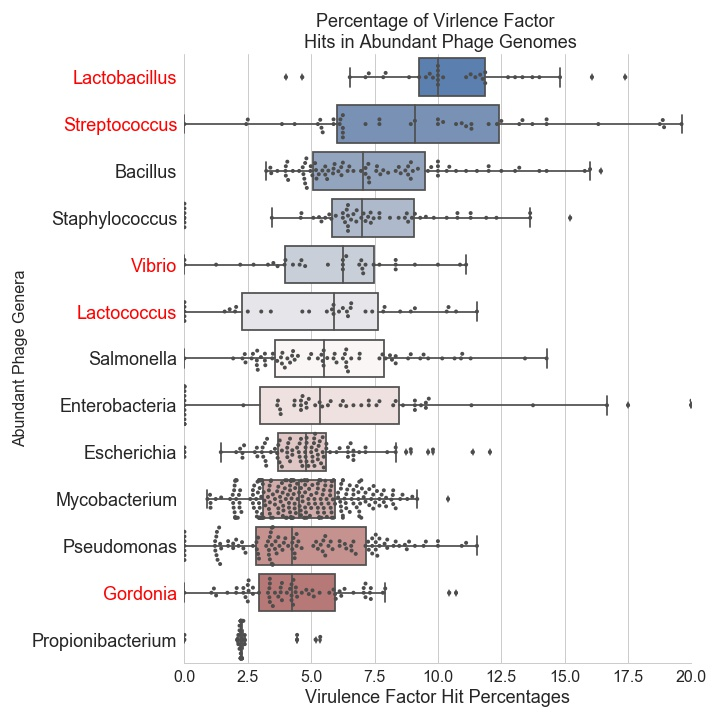
\includegraphics[height=7cm, width=8cm]{Top_Phages_Plots.jpg}
	
	\end{frame}
	
	
	\begin{frame}{Future Directions}
	\begin{block}{Magic-BLAST Streaming}
	Create a version of BUD for local metagenomic sequences 
	\end{block}
	
	\begin{block}{Testing Performance of BUD}
	Using the simulated dataset from previous study to compare the performance of identifying prophages by current tools against BUD
	\center
	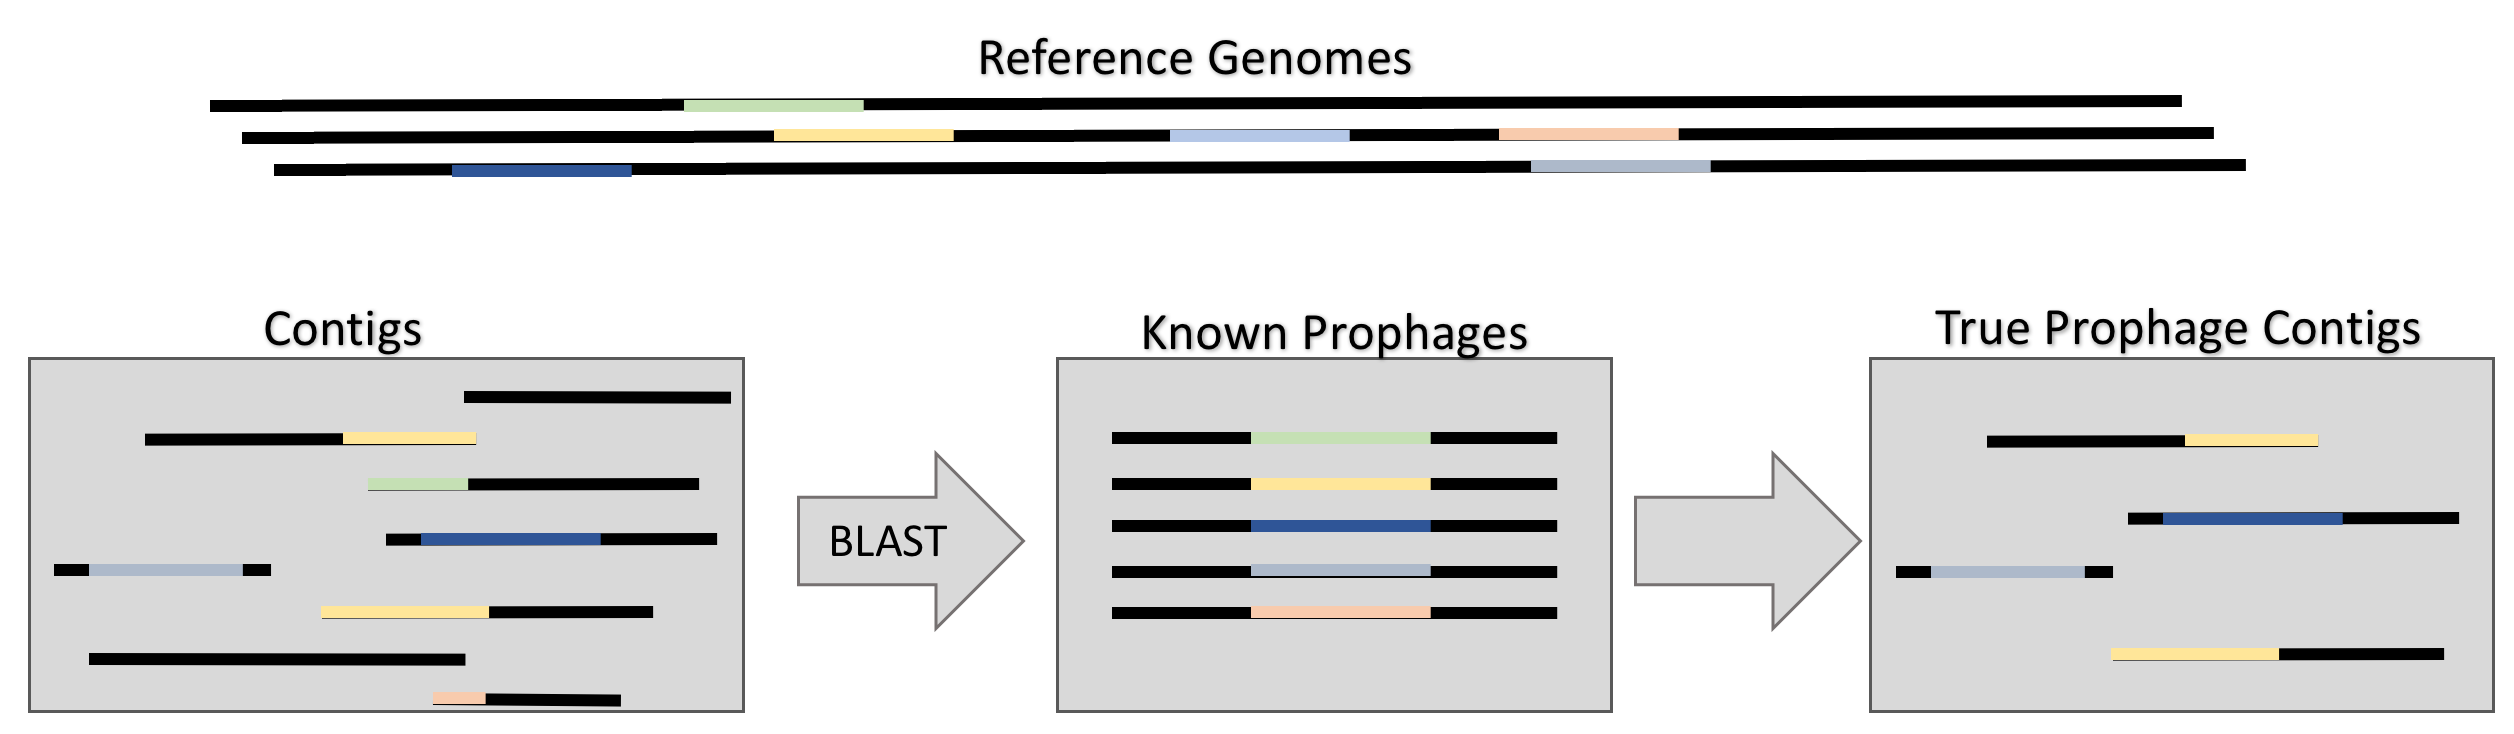
\includegraphics[height=4cm, width=8cm]{fig.png}
	
	\end{block}
	\end{frame}
	
	
\section{Hybrid Viral Contig Prediction}
\subsection{}
	\begin{frame}{Contig Prediction}

	\end{frame}
	


\section{}

	\begin{frame}{Concluding Remarks}
	\center
	
\includegraphics[height=2cm, width=10cm]{goals.png}
	\begin{columns}
	\column{0.3\textwidth}
	\begin{block}{Metagenomic Simulation Study}
	Effectively identifying viral elements improves bacterial abundance calculation
	\end{block}
	\column{0.3\textwidth}
	\begin{block}{GRAB}
	Viral GRAB will contribute to a focus on phages specific to lung infections
	\end{block}
	\column{0.3\textwidth}
	\begin{block}{Building Up Domains}
	Allows for the identification of prophages elements in metagenomics
	\end{block}
	
	\end{columns}
	
	\end{frame}
	
	
	
	
	\begin{frame}{}
	\vspace{1cm}
	{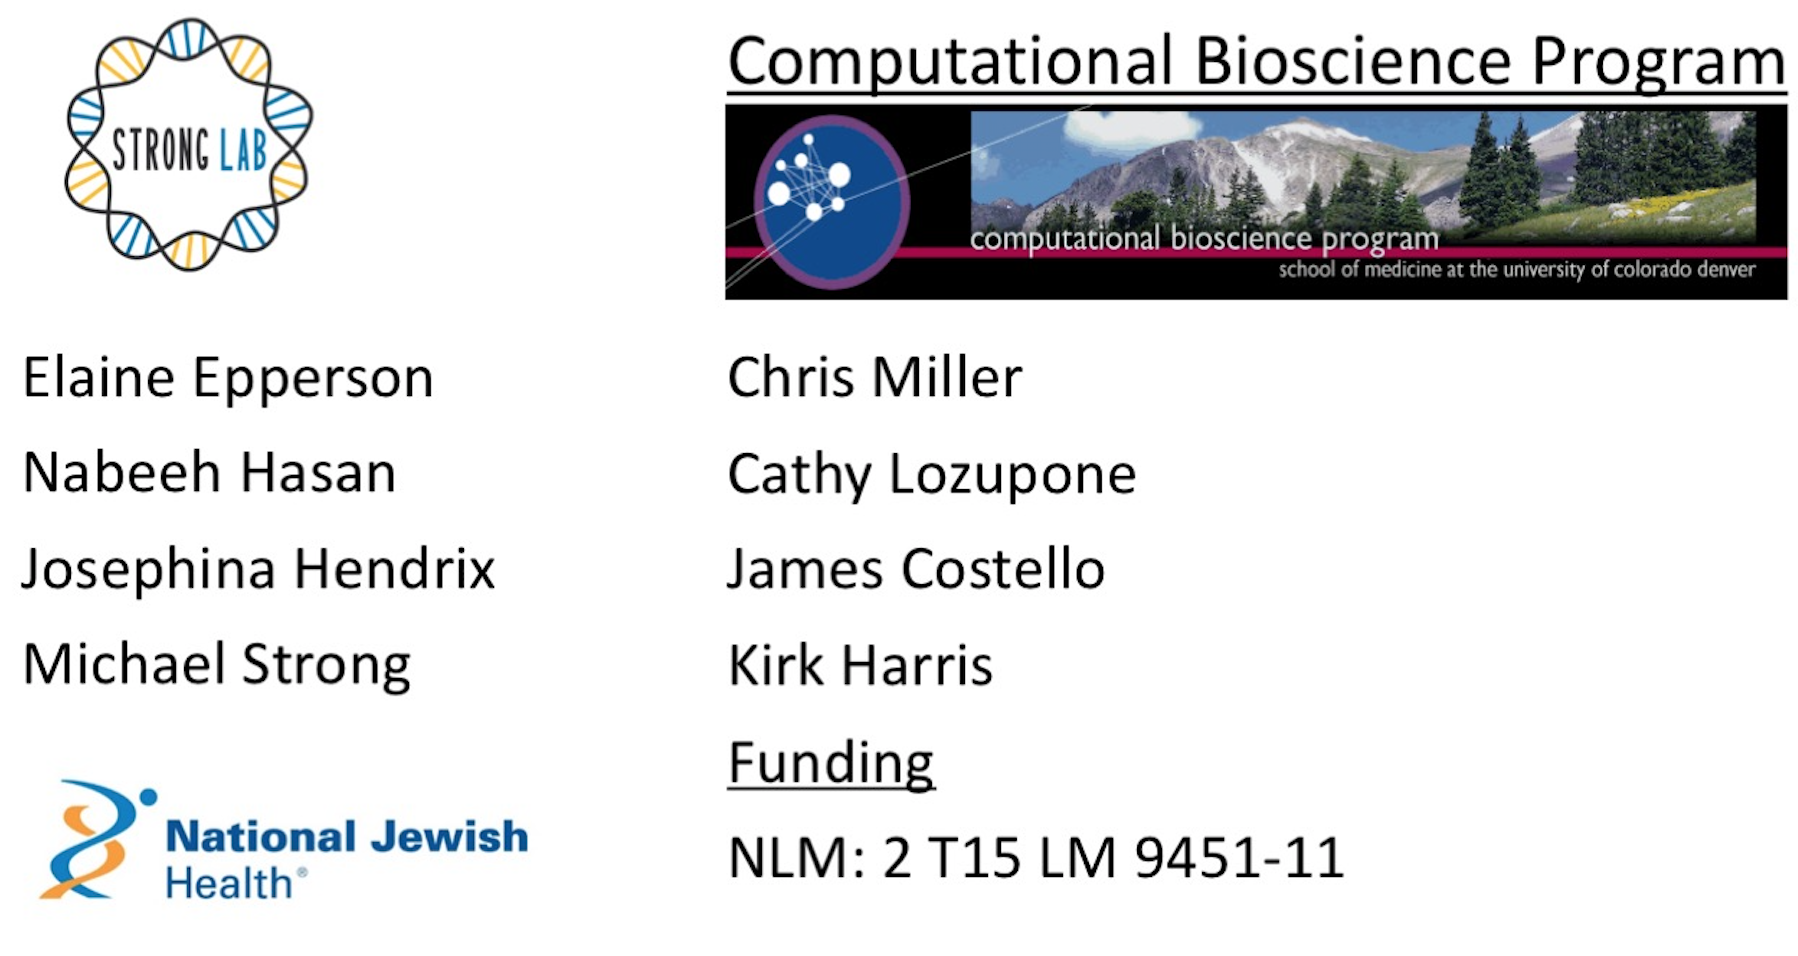
\includegraphics[height=8cm, width=11cm]{Acknowledgements.png} }
	\end{frame}
	
	
	\begin{frame}{Questions?}
	\center
	Cody Glickman \\ 
\includegraphics[height=2cm, width=2cm]{lablogo.png} \\ cody.glickman@ucdenver.edu \\ \alert{www.github.com/glickmac} \\ www.codyglickman.com
	\end{frame}
	
	
	\begin{frame}{Bias in Average Fold Coverage by GC}
	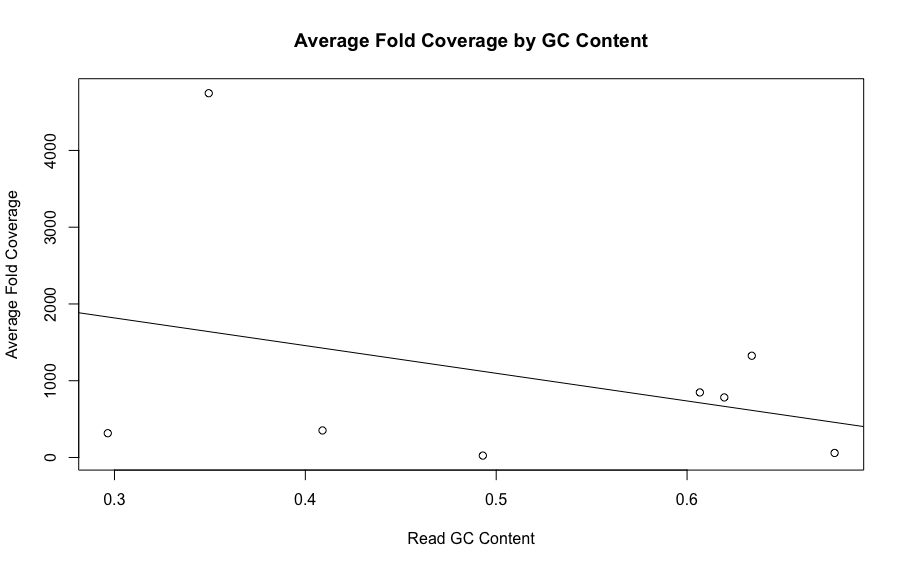
\includegraphics[height=8cm, width=11cm]{Viral_Coverage_by_GC.png}
	\end{frame}
	
	
	\begin{frame}{My Pipeline}
	\vspace{-1cm}
	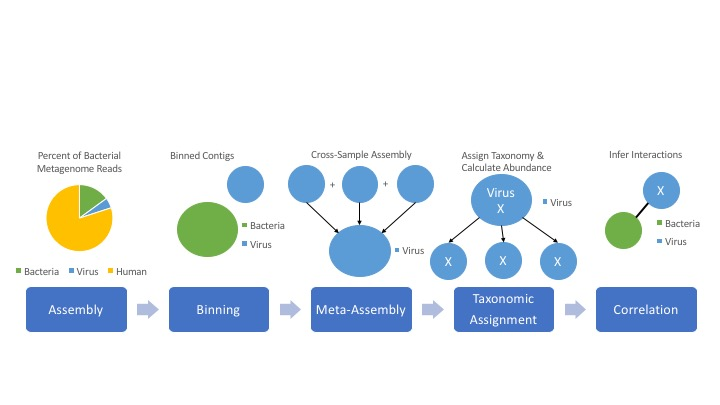
\includegraphics[height=6cm, width=11cm]{figure_2_updated.jpg}
	\end{frame}
	
	
	\begin{frame}{Tools Used in Study Continued}
	\begin{block}{Simulation Tools}
	BBMAP - a suite of tools designed for sequencing data \\
	\tiny{Bushnell, B., JGI 2016}
	\end{block}
	
	\begin{block}{Taxonomic Identification}
	Kraken - A reference-free K-mer taxonomic identifier \\
	\tiny{Wood, Derrick E., and Steven L. Salzberg Genome 2014}
	
	\large{Blastx - Referenced against a viral protein database} \\
	\tiny{Camacho C., et al. BMC Bioinformatics 2008}
	\end{block}
	
	\begin{block}{Prophage Identification}
	Phaster - A popular prophage discovery web tool  \\
	\tiny{Arndt, David, et al., Nucleic Acids Research 2016}
	\end{block}
	\end{frame}
	
	%\begin{itemize}
	%\item Prophages in bacterial reference genomes are well annotated
	%\item Location in bacterial reference genome is well annotated
	%\item find prophages in contigs and map contigs to reference.
	
	
\end{document}